\chapter{Quick summary of key points}
\label{chap:SPD_summary}

The chapters that follow would delve deeper to show more general models where variants of shifted or projected shifted partial derivatives can be used to prove lower bounds.
A lot of the lower bounds would use specific observation or tricks used in the proofs in \autoref{chap:d4-bottomfanin} and \autoref{chap:d4hom}. 

\mdfsetup{%
roundcorner=5pt
}
\begin{quote}
\begin{mdframed}
{\bf Note to reader:} All these lower bounds would involve a delicate play between the various parameters involved. In order to completely understand, it is \emph{imperative} that you work out the calculations in \autoref{chap:d4-bottomfanin} and \autoref{chap:d4hom} (specifically those in \autoref{sec:KS-leading-monomial-approach}) at least once completely. Doing that would give some sense of how the different parameters interact and this is crucial to a lot of the lower bounds that follow. 
\end{mdframed}
\end{quote}

Having said that, this chapter shall be devoted to restating the most important points to remember from the previous two chapters.
These would be enough to get a high-level view of the lower bounds that follow but one has to get their hands dirty somewhere to completely understand these.

\section{Shifted Partial Derivatives}

\begin{definition*}[Shifted Partial Derivatives, \autoref{defn:shifted-partials}]
  Let $\partial^{=k}(f)$ refer to the set of all $k$-th order partial derivatives of $f$, and $\vecx^{\leq \ell}$ refer to the set of all monomials of degree at most $\ell$. 
The \emph{shifted partials of $f$}, denoted by $\SPD{k}{\ell}{f}$, is the vector space spanned by $\inbrace{\vecx^{\leq \ell} \cdot \partial^{=k}(f)}$. 
The dimension of this space shall be denoted by $\CM{SPD}_{k,\ell}(f)$. 
\end{definition*}

\noindent
To express this pictorially, $\CM{SPD}_{k,\ell}(f)$ is the rank of the following matrix. 

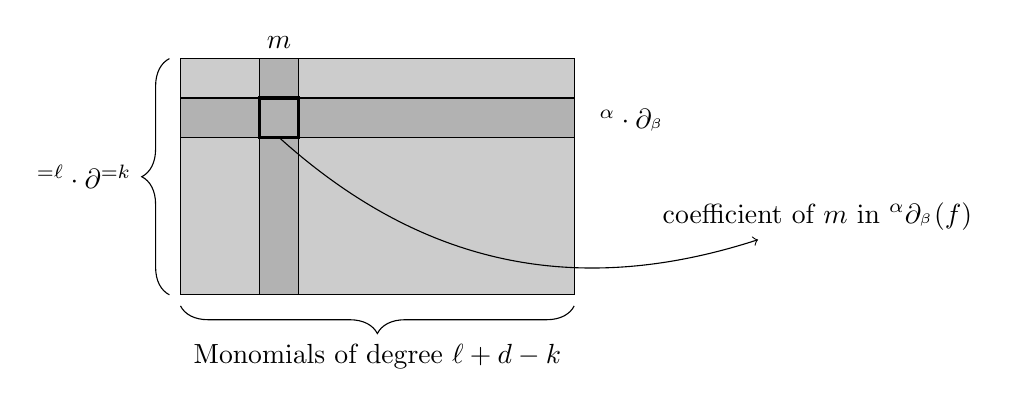
\begin{tikzpicture}
\draw[fill=black!20] (0,0) rectangle (5,3);

\draw[decorate,decoration={brace,amplitude=10pt,raise=4pt},yshift=0pt]
(0,0) -- (0,3);
\node[anchor=east] at (-0.5,1.5) {$\vecx^{=\ell} \cdot \partial^{=k}$};
\draw[decorate,decoration={brace,amplitude=10pt,mirror, raise=4pt},yshift=0pt] 
(0,0) -- (5,0);
\node[anchor=north] at (2.5,-0.5) {Monomials of degree $\ell + d - k$};

\draw[fill=black!30] (1,0) rectangle (1.5,3);
\node at (1.25,3.2) {$m$};

\draw[fill=black!30] (0,2) rectangle (5,2.5);
\node[anchor=west] at (5.2,2.2) {$\vecx^{\alpha} \cdot \partial_{\vecx^\beta}$};

\draw[very thick] (1,2) rectangle (1.5,2.5);

\node[anchor=west] at (6,1) {coefficient of $m$ in $\vecx^\alpha \partial_{\vecx^\beta}(f)$}
edge[<-,bend left] (1.25,2);
\end{tikzpicture}

This measure is used to prove lower bounds for the top fan-in of depth four circuits \emph{with bounded bottom fan-in}. 

\begin{lemma*}[Upper bound for hom. $\SPSP^{[t]}$ circuits, restating \autoref{cor:dimSPD-upper-bound}]
Let $f$ be an $n$-variate degree $d$ polynomial of the form $f = Q_1 \cdots Q_a$ with $\deg(Q_i) \leq t$. Then for any $k,\ell$, we have
\[
\CM{SPD}_{k,\ell}(f) \spaced{\leq} \binom{a}{k} \cdot \binom{n + \ell + k(t-1)}{n}
\]
\end{lemma*}

By grouping factors of degree much smaller than $t$, one can assume without loss of generality that $a = O(d/t)$.
One should note that the first binomial coefficient $\binom{a}{k}$ is at most $2^a$.
Thus if the goal is to prove a lower bound of $n^{\Omega(d/t)} = n^{\Omega(a)}$, then the first term is not too relevant. \\

\begin{exercise}
Let $H(Q_1,\ldots, Q_a)$ be an arbitrary polynomial function applied to $Q_1,\ldots, Q_a$. Suppose $\deg(Q_i) \leq t$ for all $i$. Show that
\[
\CM{SPD}_{k,\ell}(H(Q_1,\ldots, Q_a)) \spaced{\leq} \binom{a+k}{a} \cdot \binom{n + \ell + k(t-1)}{n}.
\]
\end{exercise}

The above lemma is a special case of the above more general exercise. 

The second part of the lower bound is to show that the measure is large for explicit polynomials. The Nisan-Wigderson polynomial, $\NW_{d,m,e}$, is designed so that the measure is almost as large as possible. The iterated matrix multiplication polynomial, $\IMM$, also has a large value of $\CM{SPD}_{k,\ell}$, though not as large as the value for $\NW$. For the right range of parameters, 
\[
\CM{SPD}_{k,\ell}(Q_1\cdots Q_a) \ll \CM{SPD}_{k,\ell}(\IMM) \ll \CM{SPD}_{k,\ell}(\NW) \approx \text{Maximum possible}.
\]

\section{Projected Shifted Partial Derivatives}

An important variant that shall be heavily used in the following chapters is the measure of \emph{projected shifted partial derivatives} defined in \autoref{chap:d4hom}. 

\begin{definition*}[Projected shifted partial derivatives, \autoref{defn:PSPD}]
Fix parameters $k,\ell > 0$. 
For any polynomial $P$, the set of projected shifted partials of $f$, denoted by $\mathrm{PSD}_{k,\ell}(f)$ is defined as follows
\[
\mathrm{PSD}_{k,\ell}(f) \spaced{=} \setdef{\mathrm{mult}(m_1 \cdot \partial_{m_2}(f))}{\begin{array}{c}\deg(m_1) = \ell\;,\; \deg(m_2) = k,\\ \text{$m_1$ and $m_2$ are multilinear}\end{array}}
\]
where $\mathrm{mult}(f)$ refers to the polynomial $f$ projected to only the multilinear monomials of $f$. 

The measure $\Gamma^{\mathrm{PSD}}_{k,\ell}(f)$ is defined as the dimension of the above set of polynomials, i.e.
\[\Gamma^{\mathrm{PSD}}_{k,\ell}(f) \spaced{=} \dim\inparen{\mathrm{span}(\mathrm{PSD}_{k,\ell})}\qedhere\]
\end{definition*}

Pictorially, the measure is the rank of the following matrix. 

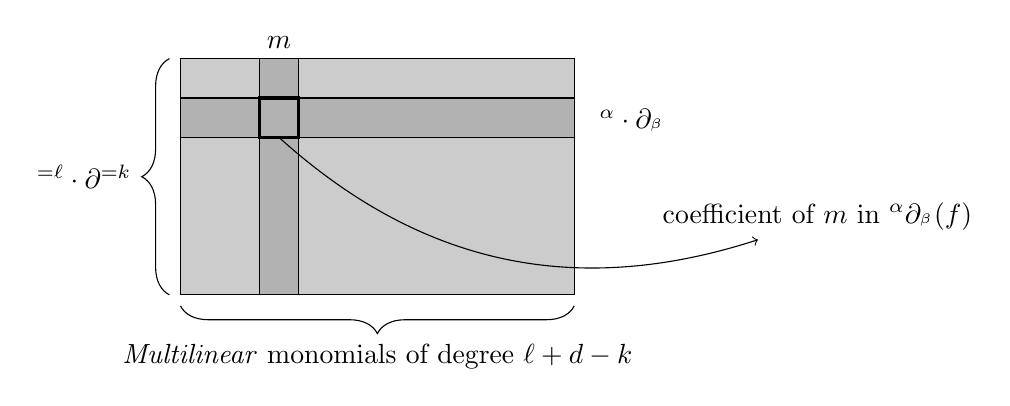
\begin{tikzpicture}
\draw[fill=black!20] (0,0) rectangle (5,3);

\draw[decorate,decoration={brace,amplitude=10pt,raise=4pt},yshift=0pt]
(0,0) -- (0,3);
\node[anchor=east] at (-0.5,1.5) {$\vecx^{=\ell} \cdot \partial^{=k}$};
\draw[decorate,decoration={brace,amplitude=10pt,mirror, raise=4pt},yshift=0pt] 
(0,0) -- (5,0);
\node[anchor=north] at (2.5,-0.5) {\emph{Multilinear} monomials of degree $\ell + d - k$};

\draw[fill=black!30] (1,0) rectangle (1.5,3);
\node at (1.25,3.2) {$m$};

\draw[fill=black!30] (0,2) rectangle (5,2.5);
\node[anchor=west] at (5.2,2.2) {$\vecx^{\alpha} \cdot \partial_{\vecx^\beta}$};

\draw[very thick] (1,2) rectangle (1.5,2.5);

\node[anchor=west] at (6,1) {coefficient of $m$ in $\vecx^\alpha \partial_{\vecx^\beta}(f)$}
edge[<-,bend left] (1.25,2);
\end{tikzpicture}

One can think of this as a sub-matrix for the shifted partial derivatives obtained by throwing out the columns corresponding to non-multilinear monomials.

This measure was used to prove lower bounds on the \emph{total size} of homogeneous depth four circuits (with no bottom fan-in restrictions), unlike the previous setting which was a top fan-in lower bound. But the following is an important note to bear in mind:
\begin{quote}
Projected shifted partial derivatives is designed to prove lower bounds on the top fan-in of homogeneous depth four circuits with \emph{low bottom support size}. 
\end{quote}
It so happens that any homogeneous depth four circuit of small total size can be reduced to a depth four circuit of small bottom support size. But this distinction is important and should be stressed. 

\subsection{Depth four circuits of low bottom support size}

Let $f = Q_1 \cdots Q_a$ with $d = \deg(f)$ and suppose all the monomials of any $Q_i$ depend on just $r$ variables.
There are two important observations made to prove the upper bound of the complexity measure on such circuits.

\begin{observation*}[Non-multiquadratic terms do not contribute]
Let $g$ be a polynomial such that every monomial of $g$ is divisible by some $x_i^3$, or in other words each monomial of $g$ is \emph{non-multiquadratic}. Then for an $k,\ell$, we have $\CM{PSD}_{k,\ell}(g) = 0$. 
\end{observation*}

\begin{observation*}[Decomposition of low support size products]
Let $f = Q_1 \cdots Q_a$ be a polynomial of degree $d$ such that all monomials of any $Q_i$ depends on at most $t$ variables. Then $f$ can be expressed as
\[
f \spaced{=} Q_1'\cdots Q_a' \spaced{+} g
\]
where $\deg(Q_i') \leq 2r$ for all $i$, and every monomial of $g$ is non-multiquadratic.
\end{observation*}

Therefore, we have
\[
\CM{PSD}_{k,\ell}(Q_1\cdots Q_a) = \CM{PSD}_{k,\ell}(Q_1'\cdots Q_a')
\]
and the RHS is a low bottom degree product. Thus similar to the upper bound for shifted partial derivatives, bearing in mind that we only care about multilinear monomials, one can easily show the following.

\begin{lemma*}[Upper bound for low bottom support size circuits, \autoref{lem:upper-bound-low-supp}]
Let $f = Q_1\cdots Q_a$ be an $n$-variate degree $d$ polynomial with each $Q_i$ a sum of monomials depending on at most $r$ variables. Then for any $k,\ell$ with $\ell + kr\leq \frac{n}{2}$, 
\[
\CM{PSD}_{k,\ell}(f) \spaced{\leq} \binom{(2d/r) + k}{k} \cdot \binom{n}{\ell + kr}
\]
\end{lemma*}

For a very delicate range of parameters, we have a very similar behaviour of the measure on the standard polynomials. 

\[
\CM{PSD}_{k,\ell}(Q_1\cdots Q_a) \ll \CM{PSD}_{k,\ell}(\IMM) \ll \CM{PSD}_{k,\ell}(\NW) \approx \text{Maximum possible}.
\]

In the right range of parameters, this gives an $n^{\Omega(d/t)}$ lower bound on the top fan-in of any homogeneous depth four circuit of bottom support size bounded by $t$ that computes $\NW$ or $\IMM$. 

The calculations involved are quite delicate but it would be useful to just keep the case of $\NW$ in mind as the full calculations were described in \autoref{sec:KS-leading-monomial-approach}. But a couple of thing to keep in mind is that the calculations for $\NW_{d,m,e}$ work over any field but as long as $m^e$ roughly equal to $2^d$ (the precise constraints are explicit described in \autoref{sec:KS-leading-monomial-approach}). \\

So far, this only addresses depth four circuits of small bottom support size. In order to reduce the general setting of homogeneous depth four circuits to this case, there is one additional trick employed. 

\subsection{Reducing  to depth four circuits of low bottom support size}

The key observation here is that if we have a depth four circuit of small size, then the number of distinct monomials computed at the layer closest to the leaves is bounded by the size of the circuit.
As a concrete instance, say we have a depth four circuit of size $s = n^{(0.1) \sqrt{d}}$.
We shall now pick a \emph{lot} of variables at random and set them to zero or to be more precise we shall set each variable to $0$ independently with probability $1 - \frac{1}{n^{0.2}}$. With very high probability, we would now be left with about $n^{0.8}$ variables but the resulting circuit remains homogeneous as setting variables to zero maintains homogeneity. 

However, if $m$ is a monomial that depends on $\sqrt{d}$ or more variables, the probability that this monomials survives this random restriction is at most $\frac{1}{n^{(0.2) \sqrt{d}}}$. Thus, even if we union bound over all monomials present in the depth four circuit of size $n^{(0.1)\sqrt{d}}$ we get
that the probability that some monomial of support $\sqrt{d}$ or more survives this process is at most $\frac{1}{n^{(0.1)\sqrt{d}}} = o(1)$. Thus, almost surely, the resulting circuit is now a homogeneous depth four circuit with bottom support size at most $\sqrt{d}$. \\

This however complicates the other side of the argument where we now need to find a polynomial $P$ such that \emph{even after a random restriction $\rho$ is applied on $P$}, we must have $\CM{PSD}_{k,\ell}(\rho(P))$ to be large. This is extremely non-trivial to see if $\NW$ or $\IMM$ are so robust. Fortunately, there is a hack that allows us to circumvent this at the cost of making the polynomial uglier. 

\begin{lemma*}[Linear blow-up trick to handle random restrictions, \autoref{lem:lin-transform-trick}]
Let $\rho$ be a random restriction that sets each variable to zero independently with probability $1 - \alpha$. 
For any polynomial $P(x_1,\dots x_n)$, define $P \circ \mathrm{Lin}_\alpha$ as
\[
P \circ \mathrm{Lin}_\alpha \spaced{=} P\inparen{\sum_{i=1}^t y_{1i}, \ldots, \sum_{i=1}^t y_{nt}}\quad \text{where $t = \inparen{\frac{1}{\alpha}} n \log n$}
\]
Then, $\rho(f \circ \mathrm{Lin}_\alpha)$ has $f$ as a projection with probability $1 - 1/2^{n}$. 
\end{lemma*}

Basically, we replace each variable in $\NW$ by a sum of $t$ new distinct variables where $t = (1/\alpha) \log n$. The point is that, if a variable is kept alive with probability $\alpha$, then with very high probability, one of the $t$ variables $\set{y_{ij}}_{j\in [t]}$ will be kept alive for each $x_i$. Hence, there is a copy of $\NW_{d,m,e}$ sitting inside $\rho(\NW_{d,m,e} \circ \mathrm{Lin}_\alpha)$ with very high probability. 

Therefore, if we assume on the contrary that $C$ is a homogeneous depth four circuit of size $n^{(0.1)\sqrt{d}}$ computing $\NW_{d,m,e} \circ \mathrm{Lin}_\alpha$, then there is a homogeneous circuit $C'$ with size at most $n^{(0.1)\sqrt{d}}$ and bottom support size at most $\sqrt{d}$ that computes $\NW_{d,m,e}$. But since we already have a lower bound for homogeneous depth four circuits of low bottom support size computing $\NW_{d,m,e}$, we get a contradiction. \\

Hopefully this would give the readers a rough description of the main observations. But to really understand them, one \emph{has} to work out the calculations in \autoref{sec:KS-leading-monomial-approach} at least once to get a better grip of how these parameters interact. We now move on to some other models for which projected shifted partials, or variants of it, can again be employed. 


%%% Local Variables:
%%% mode: latex
%%% TeX-master: "fancymain"
%%% End:
